\section{\os-Level Task-Based Mechanism for Lightweight Manycore Processors}
\label{sec:solution}

	% Overview
	The proposed \textit{task} abstraction can be seen as a special case of
	coroutines.  It encapsulates a subroutine that can be performed regardless
	of who created them. However, unlike coroutines, the proposed task
	definition is disconnected from the need to have a dedicated thread per
	task. At this point, we introduce a special thread, named
	\textit{dispatcher}, which is a generic task executor. Following the
	producer-consumer model, the dispatcher consumes tasks from a global task
	queue, where requesters atomically insert tasks to be performed.

	\begin{algorithm}[b]
		\label{alg:dispatcher}
		\While{Not shutdown}{
			Waits for a task\;
			Execute task function\;
			\Switch{Task return}{
				\Case{TASK\_RET\_SUCCESS}{
					Complete the task and schedule children\;
				}
				\Case{TASK\_RET\_AGAIN}{
					Reschedule the task\;
				}
				\Case{TASK\_RET\_STOP}{
					Insert the task into a waiting queue\;
				}
				\Case{TASK\_RET\_ERROR}{
					Propagate the error and release all tasks\;
				}
			}
		}
		\caption{How to write algorithms}
	\end{algorithm}

	A \textit{task} is a standardized structure that holds semantic and control
	information. On the one hand, the semantic variables store the function to
	be performed, its arguments, and a slot to store the return value. On the
	other hand, control variables, referring to the semantics of the
	dispatcher, are composed of the state of the task, a list of dependent
	tasks, the number of active parent tasks, and a synchronization control
	with the requester. This allows the creation of dependency graphs that
	introduce more sophisticated managements and asynchronous behaviors. These
	dependencies guarantee that a task will only be ready to execute when all
	the parent tasks have completed their executions.

	Pseudocode~\ref{alg:dispatcher} summarizes the behavior of a dispatcher.
	Blocked at a semaphore, the dispatcher will wait for new task requests to
	appear. When consuming a task, the dispatcher updates its state and begins
	executing the task scope. At this point, it is possible to notice the reuse
	of a stack of the dispatcher for numerous independent tasks. Specifically,
	when it returns from the task scope, it will be in its initial state and
	able to start another task.	This algorithm supports the spawn of more than one
	dispatcher that will cooperate to handle the tasks. It will increase the
	parallelism and decrease the waiting time but required more memory pages.
	The task can also signal the completion status to the dispatcher between
	three values. Specifically:

	\begin{description}
		\item[TASK\_RET\_SUCCESS] the dispatcher will complete the task,
			signaling its completion to child tasks and releasing the
			requester.
		\item[TASK\_RET\_AGAIN] The task returned with an error but is
			recoverable and the task will be rescheduled.
		\item[TASK\_RET\_STOP] The task returned with an error, but despite
			being recoverable, it needs to wait for another operation to
			resume.
		\item[TASK\_RET\_ERROR] The task returned an error and is
			unrecoverable, the dispatcher will signal the error to the
			requester and propagate the error to all child tasks.
	\end{description}
	% Problem address
	The proposed task-based mechanism at the \os-level addresses the problems
	described in the previous section as follows:
	%
	\begin{description}
		\item[Memory Utilization] The definition of multiple execution streams
			in isolated tasks, or in a dependency graph, reduces the use of
			memory pages for threads based on the number of existing
			dispatchers. If the kernel and the application are able to isolate
			simple behaviors without the need to create a dedicated thread,
			more memory will be available to store useful data.

		\item[Data Locality] Configuring a dispatcher to always be in only the
			same core, it can perform tasks that share the same data structures
			by exploring the location of the data cache.

		\item[Core Utilization] This a significant point to define the
			dispatcher at the \os-level that makes it possible to move it to the
			master core. Therefore, it will share the execution time with the
			master thread. At one extreme, we could even define the master
			thread itself has a dedicated dispatcher.

		\item[Asynchronous Operations] Modeling tasks to move the
			responsibility to send the data to the dispatcher, introduce this
			notion of asynchronous send/read. The same idea applies to
			syscalls, where non-critical operations can be performed
			asynchronously.

		\item[Periodic Operations] Tasks can be modeled to have a period to
			which they are unblocked and operate. In this way, we eliminate the
			need to have a dedicated thread that is waiting for some condition
			to carry out specific operations. For example, reading
			a communication from the \noc that will create a new task to execute
			a remote procedure.
	\end{description}

	\begin{figure}[tb]
			\centering
			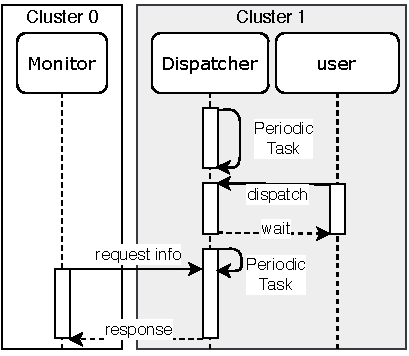
\includegraphics[width=0.6\linewidth]{monitoring}
			\caption{Clusters interations using tasks.}
			\label{fig:monitor}
	\end{figure}

	Figure~\ref{fig:monitor} illustrates the interactions within the kernel
	after implementing the task mechanism. Periodic tasks created by the kernel
	allowed for a richer intra- and inter-cluster interaction. As the master
	thread responsible for handling one request at a time, moving that
	responsibility to the dispatcher will not introduce a bottleneck in the
	system beyond what already exists. Finally, tasks requested by ordinary
	users can and should be interleaved, which leads to the need for
	finer-grain management than a simple insertion in a queue.	

